\section{Related Work - Activity Forecasting}

\begin{frame}
	\frametitle{Related Work}
	\framesubtitle{Activity Forecasting through Semantic Mapping}
	
	\vspace{0.33cm}
	
	\large
	
	\textbf{Ziebart \emph{et al.} \cite{Kitani12}} propose a method for activity forecasting by
	combining:
	
	\begin{itemize}
		\item Semantic scene understanding
		\vspace{0.05cm}
		\item Inverse Optimal Control
	\end{itemize}
	
	\vspace{-0.2cm}
	
	\begin{center}
		\begin{tikzpicture}
			\node at (0,0) [draw=white,ultra thick,inner sep=0pt]
			{
				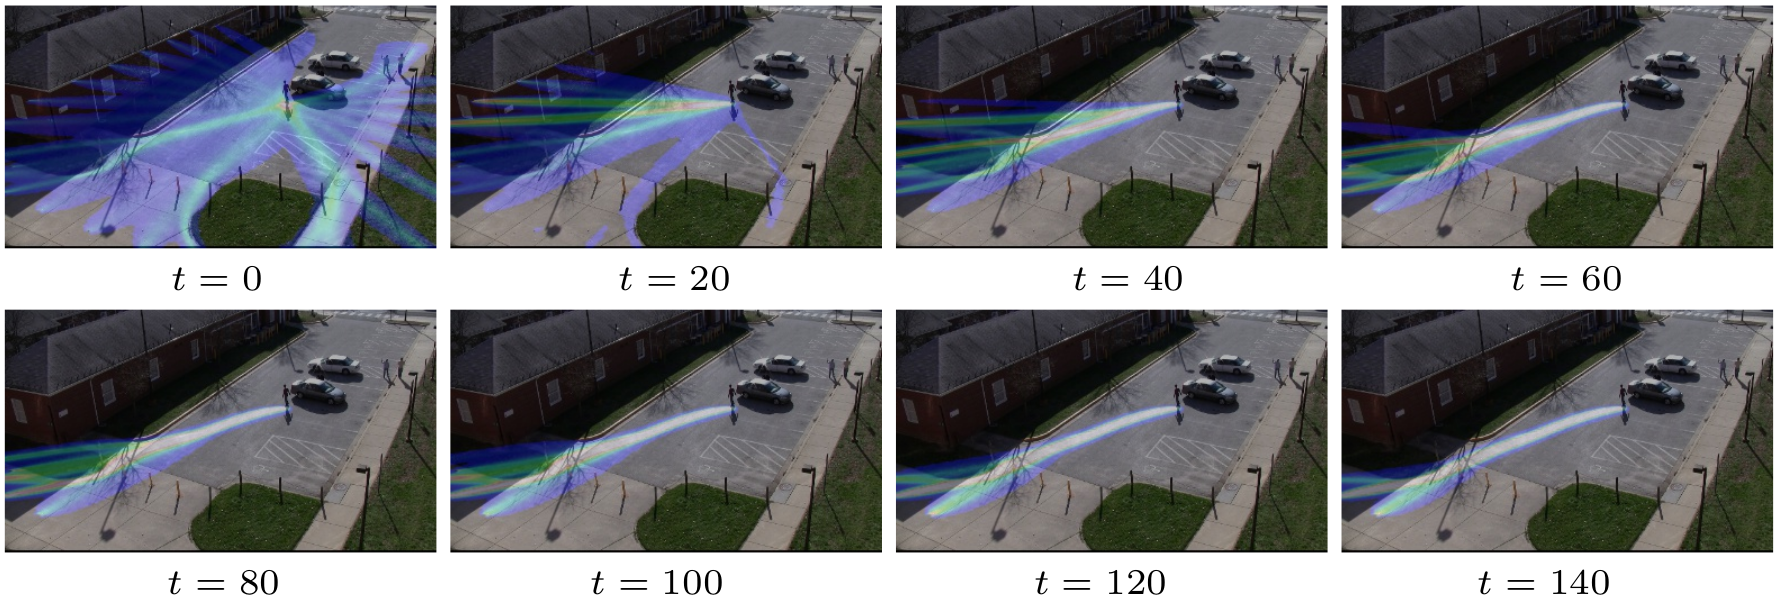
\includegraphics[scale=0.19]{Figures/ActivityForecasting.png}
			};
		\end{tikzpicture}
	\end{center}
	
	\vspace{-0.3cm}
	
	\tiny
	
	\cite{Kitani12} B. D. Ziebart \emph{et al.}, ``Activity forecasting'', ECCV, 2012
\end{frame}

\begin{frame}
	\frametitle{Advantages/Disadvantages}
	
	\Large
	
	\vspace{0.4cm}
	
	\underline{\textbf{Advantages}} \\
	
	\vspace{0.2cm}
	
	\begin{itemize}
		\item Knowledge transfer by using physical scene features
		\item Accurate and robust destination forecasting
	\end{itemize}
	
	\vspace{0.2cm}
	
	\underline{\textbf{Disadvantages}} \\
	
	\vspace{0.19cm}
	
	\begin{itemize}
		\item Prior knowledge of potential goals
		\item Applicability in dynamic environments? \\
			  \vspace{-0.2cm}
			  \begin{tabbing}
				  \hspace{0.3cm}
				  \large
				  $ \leadsto $ \emph{rescue or rapidly changing construction environment}
			  \end{tabbing}
	\end{itemize}
\end{frame}
